\documentclass{article}
\usepackage[margin=1in]{geometry}
\usepackage[utf8]{inputenc}
\usepackage[english]{babel}
\usepackage{amssymb}
\usepackage{amsmath}
\usepackage{gensymb}
\usepackage{graphicx}
\usepackage{ragged2e}
\usepackage{blindtext}
\usepackage{setspace}
\usepackage{tabularx}
\setlength{\parindent}{4em}
\setlength{\parskip}{1em}
\renewcommand{\baselinestretch}{1.0}

\begin{titlepage}
\clearpage\thispagestyle{empty}
\title{%
   \large{Univerzita Karlova}\\
    \vspace{1cm}\\
   \large{Přírodovědecká fakulta}\\
\vspace{2cm}\\
\[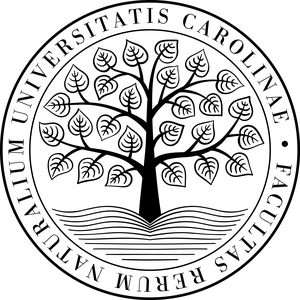
\includegraphics[height=60mm]{images/logo_uk.PNG}\]
\vspace{2cm}\\
   \Large{Úloha 3 - Digitální model terénu}\\
   \vspace{1cm}\\
  \large{Algoritmy počítačové kartografie}
\vspace{3cm}\\
    \large{Tomáš Hřebec, Kateřina Obrazová}\\
    \date{Praha 2022}}
\end{titlepage}
\begin{document}
\maketitle
\thispagestyle{empty}
\doublespacing
\section{\large{Zadání úlohy}}
\subsection{\small{Povinná část}}
\justifying
\textit{Vstup: Množina $P = \{p_{1}, ..., p_{n}\}$, $p_{i} = \{x_{i}, y_{i}, z_{i}\}$.}
\vspace{0.2cm}\\
\textit{Výstup: polyedrický DMT nad množinou P představovaný vrstevnicemi doplněný vizualizací sklonu trojúhelníků a jejich expozicí.}
\vspace{0.2cm}\\
Metodou inkrementální konstrukce vytvořte nad množinou P vstupních bodů 2D Delaunay triangulaci. Jako vstupní data použijte existující geodetická data (alespoň 300 bodů) popř. navrhněte algoritmus pro generování~syntetických vstupních dat představujících významné terénní tvary (kupa, údolí, spočinek, hřbet,~...).
\vspace{0.2cm}\\
Vstupní množiny bodů včetně níže uvedených výstupů vhodně vizualizujte. Grafické rozhraní realizujte s využitím frameworku QT. Dynamické datové struktury implementujte s využitím STL.
\vspace{0.2cm}\\
Nad takto vzniklou triangulací vygenerujte polyedrický digitální model terénu. Dále proveďte tyto analýzy:\begin{itemize}
    \item S využitím lineární interpolace vygenerujte vrstevnice se \textit{zadaným~krokem} a v \textit{zadaném~intervalu}, proveďte jejich vizualizaci s rozlišením zvýrazněných vrstevnic.
    \item Analyzujte sklon digitálního modelu terénu, jednotlivé trojúhelníky vizualizujte v závislosti na jejich sklonu.
    \item Analyzujte expozici digitálního modelu terénu, jednotlivé trojúhelníky vizualizujte v závislosti na jejich expozici ke světové straně.
\end{itemize}
Zhodnoťte výsledný digitální model terénu z kartografického hlediska, zamyslete se nad slabinami algoritmu založeného na 2D Delaunay triangulaci. Ve kterých situacích (různé terénní tvary) nebude dávat vhodné výsledky? tyto situace graficky znázorněte.
\vspace{0.2cm}\\
Zhodnocení činnosti algoritmu včetně ukázek proveďte alespoň na \textbf{3 strany} formátu A4.
\subsection{\small{Volitelná část}}
Barevná hypsometrie.
\clearpage
\newpage
\section{\large{Popis problému}}
Terén je 2-rozměrný povrch ve 3-rozměrném prostoru se speciální vlastností - každá svislá jej protíná v bodě, pokud jej vůbec protíná, tj. graf funkce $f: A \in R^2 \rightarrow R$, který přiřazuje výšku $f(p)$ každému bodu $p$ v oblasti terénu $A$. V globálním měřítku takto definovaný terén není dobrým modelem Země, avšak v lokálnějším měřítku poskytuje dobré modely. (de Berg a kol. 2008)
\subsection{\large{Triangulace}}
Ve 2D probíhá klasická triangulace tak, že je množina bodů $p_{i} \in P$, které budou spojeny hranami $e_{i} \in E$ tak, že tyto hrany budou tvořit trojúhelníky $t_{i} \in T$. Tyto hrany a trojúhelníky lze považovat množiny dvou nebo tří bodů. Cílem triangulačního procesu je vytvořit z daných bodů jednotnou geometrickou entitu $P$, která má podobu trojúhelníkové sítě. (Bærentzen a kol. 2012)
\subsection{\large{Delaunayho triangulace}}
Delaunayho triangulace byla zavedena v roce 1934. (Delaunay 1934) Delanay dokázal, že pokud je duální graf nakreslen rovnými čarami, vytvoří tím rovinnou triangulaci Voroniových míst $P$ (pokud žádná 4 místa nejsou kocirkulární). Delaunayova triangulace ve 2D lze rozšířit na 3D, kde se stává Delaunayovou tetrahedronizací. (Bærentzen a kol. 2012)\\
Nechť $P$ je množina bodů (či míst) $P$ v rovině. Z definice Voroného diagramu se ví, že dělí rovinu na $n$ oblastí, tedy oblast místa $p \in P$ obsahuje všechny body $p$, pro které je $p$ nejbližším místem. Voroného diagram množiny bodů $P$ nazveme Vor($P$). Oblast místa $p$ nazýváme Voroného buňkou místa $p$ a označíme ji $\mathcal{V}(p)$. (de Berg a kol. 2008)
Nyní bude zkoumán duální graf Voroného diagramu $\mathcal{G}$, který má uzel pro každou Voroného buňku (ekvivalentně pro každé místo) a má oblouk mezi dvěma uzly, pokud odpovídající buňky sdílejí hranu. Z Obrázku 1 je patrné, že $\mathcal{G}$ má oblouk pro každou hranu Vor($P$) a existuje vzájemná shoda mezi ohraničenými plochami $\mathcal{G}$ a vrcholy Vor($P$). (de Berg a kol. 2008) \\
\[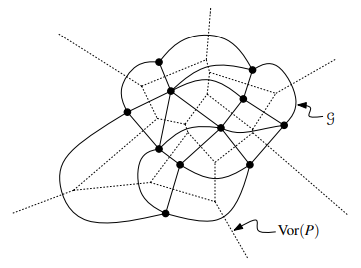
\includegraphics[height=50mm]{images/voro_1.PNG}\]
\[\textit{\footnotesize{Obr. 1 - Voroného duální graf Vor($P$)}}\]
\textit{„Uvažujeme-li přímkové vnoření $\mathcal{G}$, kde uzel odpovídající Voroného buňce $\mathcal{V}(P)$ je bod $p$ a oblouk spojující uzly $\mathcal{V}(p)$ a $\mathcal{V}(q)$ je $\overline{pq}$ (de Berg a kol. 2008)."} (Obr. 2)
\[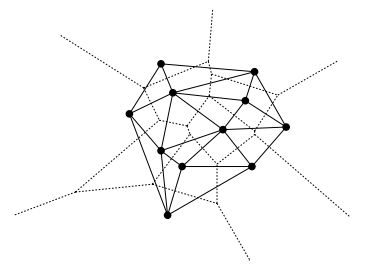
\includegraphics[height=50mm]{images/voro_2.PNG}\]
\[\textit{\footnotesize{Obr. 2 - Delaunayho graf $\mathcal{DG}(P)$}}\]
Níže jsou uvedeny definice pojmů spojené s Delaunayovou triangulací:\\
%---------------------------definice----------------------------------
\textit{\textbf{Prázdný kruh}: „Kruh je prázdný právě tehdy, když jeho vnitřek neobsahuje žádné body $P$.“}
\vspace{0.2cm}\\
\textit{\textbf{Kružnice opsaná na hraně}: „Kružnice opsaná na hraně od $p_{i}$ do $p_{j}$ je kružnice procházející skrz $p_{i}$ a $p_{j}$.}
\indent\indent\indent\indent\indent\indent\indent\indent\indent\textit{~Pro každou hranu existuje nekonečně mnoho kružnic opsaných.“}
\vspace{0.2cm}\\
\textit{\textbf{Delaunayova hrana}: „Hrana je Delaunayova pouze tehdy, má-li prázdnou kružnici opsanou.“} (Obr. 3)\\
\[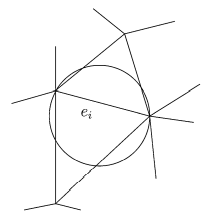
\includegraphics[height=45mm]{images/del_hrana.PNG}\]
\[\textit{\footnotesize{Obr. 3 - Příklad, kdy hrana $e_{i}$ je Delaynayova}}\]
\textit{\textbf{Delaunayova triangulace}: „Triangulace $\mathcal{D}$ je Delaunayovou triangulací, jestliže hrana je Delaunayova}
\indent\indent\indent\indent\indent\indent\indent\indent\indent\textit{právě tehdy a jen tehdy, když je v $\mathcal{D}$. To je Delaunayova triangulace množiny}
\indent\indent\indent\indent\indent\indent\indent\indent\indent\textit{bodů jsou všechny Delaunayovy hrany související s těmito body.“}\\
„\textit{Tato definice je ve vztahu k triangulaci naprosto smysluplná pouze tehdy, pokud žádné čtyři body v $P$ neleží na společné kružnici a žádné tři body v $P$ nejsou zarovnány.“}\\
\vspace{0.2cm}\\
\textit{\textbf{Kružnice opsaná trojúhelníku}: „Kružnice opsaná trojúhelníku je jedinečná kružnice procházející jeho třemi vrcholy.“} (Obr. 4)\\
\[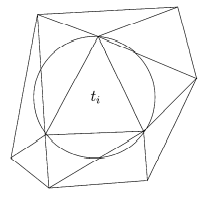
\includegraphics[height=40mm]{images/del_troj.PNG}\]
\[\textit{\footnotesize{Obr. 4 - Příklad, kdy trojúhelník $t_{i}$ je Delanayův}}\]
\textit{\textbf{Delaunayho trojúhelník}: „Trojúhelník je Delaunayův jen a pouze když kružnice opsaná je prázdná.“}
\indent\indent\indent\indent\indent\indent\indent\indent\textit{~~~(Bærentzen a kol. 2012, str. 243)}
\subsection{\large{Sklon}}
Sklon (\emph{angl. slope}) je veličina, která udává sklon křivky nebo čáry vzhledem k jiné křivce či přímce. Pro přímky v rovině xy svírající s osou x úhel $\Theta$ je sklon $m$ konstanta daná vztahem
\[ m = \frac{\Delta y}{\Delta x} = \textrm{tg} \Theta,\]
kde \begin{itemize}
    \item $\Delta y$ a $\Delta x$ jsou změny dvou souřadnic o určitou vzdálenost. (Weisstein 2016)
\end{itemize}
\subsection{\large{Expozice}}
Expozice, neboli orientace svahu \emph{(angl. aspect)} popisuje orientaci povrchu vůči světovým stranám. Vyjadřuje se ve stupních v rozsahu 0$\degree$–360$\degree$. Není definována v singulárních bodech (vrchol, sedlo aj.). Orientace v bodě je definována jako azimut průmětu gradientu do roviny xy.
\clearpage
\newpage
\section{\large{Dokumentace}}
Program je rozdělen do 7 modulů. Modul \emph{Mainform.py} je převážně vygenerován pomocí softwaru QT Creator a slouží k vytvoření uživatelského rozhraní (Obr. 5). Modul \emph{algorithm.py} obsahuje algoritmy pro tvorbu a analýzu TIN. Modul \emph{draw.py} slouží především pro propojení předešlých dvou modulů, k zajištění vizualizace vstupu a výstupu. Modul \emph{input.py} zajišťuje nahrání vstupních dat v požadovaném formátu. Modul \emph{qpoint3d.py} upravuje třídu \texttt{QPoint}tak, aby v sobě nesla informaci i o souřadnici Z. Modul \emph{edge.py} definuje třídu \texttt{Edge}, která definuje datový typ hrany. Hrana v sobě nese informaci o počátečním a koncovém bodě. Poslední modul \emph{settings.py} je opět vytvořen v softwaru QT Creator a umožňuje vyvolání dialogového okna v uživatelském rozhraní.
\[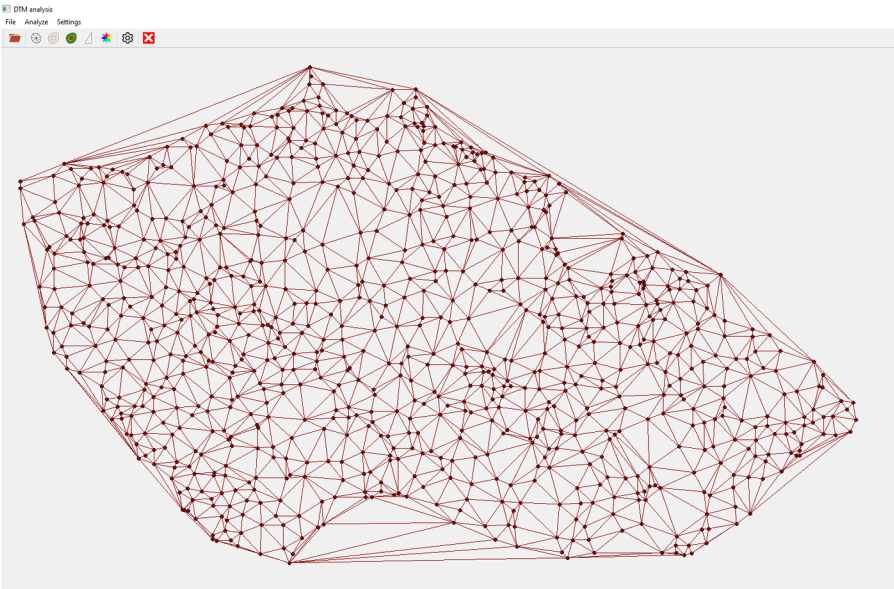
\includegraphics[height=110mm]{images/nahled_DTM.PNG}\]
\[\textit{\footnotesize{Obr. 5 - Náhled uživatelského rozhraní}}\]
\subsection{\small{Modul Mainform.py}}
Tento modul obsahuje třídu \texttt{Ui\_Mainform} která je vytvořena automaticky pomocí QT Creatoru. Tato třída byla posléze doplněna o metody, které se spustí při interakci s uživatelským rozhraním. Jedná se o metody \emph{runDT, runContourLines, openFile, computeSlope, computeAspect, createColorH, clearAll, clearCL, clearSlope, clearAspect, clearColorH} a \emph{showSettings}. Metoda \emph{openFile} vyvolá funkci \emph{loadFile} z modulu \emph{input.py} a tím nahraje vstupní body ze shapefilu do proměnné \emph{points} ve třídě \texttt{Draw}. Metoda \emph{runDT} zajišťuje volání zvoleného algoritmu pro tvorbu Delaunayho triangulace. Výsledná triangulace je uložena do listu v podobě jednotlivých hran ve třídě \texttt{Draw}. Metoda \emph{runContourLines} vytvoří vrstevnice na základě Delaunayho triangulace. Parametry pro tvorbu vrstevnic jsou načteny z uživatelského rozhraní pomocí modulu \emph{settings.py}. Vrstevnice jsou uloženy v listu ve formě hran v třídě \texttt{Draw}. Metoda \emph{computeSlope} vypočte sklon jednotlivých trojúhelníku Delaunayho triangulace a uloží jej do listu ve třídě \texttt{Draw}. Metoda \emph{computeAspect} vypočte orientaci jednotlivých trojúhelníků Delaunayho triangulace a uloží jej do listu ve třídě \texttt{Draw}. Metoda \emph{createColorH} vypočte průměrnou nadmořskou výšku jednotlivých trojúhelníků Delaunayho triangulace a uloží jej do listu ve třídě \texttt{Draw}. Metody \emph{clearAll, clearCL, clearSlope, clearAspect} a \emph{clearColorH} mažou listy z daty ve třídě \texttt{Draw}. Poslední metoda \emph{showSettings} vyvolá dialogové okno uživatelského rozhraní pro nastavení parametrů pro tvorbu vrstevnic.
\subsection{\small{Modul input.py}}
Tento modul obsahuje metodu \emph{loadfile}. V této metodě nejprve načtena cesta ke vstupním datům. Když není zvolena žádná cesta, metoda se ukončí. Dále je načten vstupní shapefile. Data z tohoto shapefilu jsou převedeny do formátu \emph{QPoint3D}, který je schopen nést i informaci o nadmořské výšce z bodu. Nadmořská výška je odečtena z atributů bodů, které se nacházejí v atributové tabulce shapefilu. Následně tyto data musejí být ještě zobrazena do lokálního souřadnicového systému, který je definován velikostí okna. Takto transformovaná data jsou poté jako jednotlivé body vloženy do listu \emph{points}, který je posléze touto metodou vracen. Metoda také vrací měřítko \emph{scale}, které nese informaci o změně velikosti os x a y.
\subsection{\small{Modul draw.py}}
Tento modul obsahuje třídu \emph{Draw}, kterou dědí od třídy \texttt{QWidget} z knihovny PyQt6. Hlavní funkce tohoto modulu je vykreslovat vstupní body a následně výsledky jednotlivých funkcí. Body jsou uloženy v listu \emph{points}. Výsledky funkcí jsou poté uloženy v listech \emph{dt} (výsledky triangulace), \emph{cont\_lines} (vrstevnice), \emph{heights} (nadmořská výška trojúhelníků), \emph{slope} (sklon trojúhelníků), \emph{aspect} (orientace trojúhelníků). Toto vykreslení je definováno v metodě \emph{paintEvent}.\\
Poslední metody jsou jednotlivé \emph{gettery} a \emph{settery} pro editaci dat z ostatních modulů.
\subsection{\small{Modul algorithm.py}}
Zde se nacházejí jednotlivé algoritmy pro tvorbu digitálního modelu terénu. V modulu se nachází jediná třída \texttt{Algorithms}, která obsahuje jednotlivé potřebné metody, pro tvorbu digitálního modelu terénu.\\
Metoda \emph{getPointAndLinePosition} má a vstupu 3 body \emph{QPoint3D}, kde 2 definují přímku a 1 analyzovaný bod. Tato metoda zjistí, ve které polorovině se analyzovaný bod nachází. Výsledek je vracen jako 1 pro bod v levé polorovině, -1 pro bod v pravé polorovině a 0 pro kolineární bod.\\
Metoda \emph{get2LinesAngle} má na vstupu 4 body \emph{QPoint3D}, kde první 2 definují první úsečku a druhé 2 definují druhou úsečku. Výstupem této metody je úhel mezi dvěma úsečkami v radiánech.\\
Metoda \emph{getCircleCenterAndRadius} má na vstupu 3 body \emph{QPoint3D}, které definují výslednou kružnici. Z daných 3 bodů jsou vypočteny souřadnice středu kružnice a její poloměr. Střed kružnice je vracen jako \emph{QPoint3D} a poloměr jako \emph{float}.\\
Metoda \emph{getNearesPointIdx} má na vstupu bod \emph{QPoint3D} a list všech bodů \emph{QPoint3D}. Metoda projde všechny body v listu a nalezne nejbližší netotožný bod k zadanému bodu. Tento index je vracen jako \emph{int}.\\
Metoda \emph{getDelaunayPointIdx} má na vstupu hranu \emph{Edge} a list bodů \emph{QPoint3D}. Metoda nalezne optimální bod k hraně tak, že projde všechny vstupní body (kromě identického bodu s body definující hranu) a vybere bod, který společně body hrany vytváří kružnici s nejmenším poloměrem. Body v levé polorovině jsou preferovány nad body v pravé. Funkce vrací index optimálního bodu. Když není žádný bod optimální, je vracena hodnota -1.\\
Metoda \emph{DT} ze vstupních bodů vytváří Delaunayho triangulaci. Tuto triangulaci vrací jako list jednotlivých hran \enph{Edge}. Podrobný popis algoritmu je popsán níže v pseudokódu.\\
Metoda \emph{updateAEL} má na vstupu hranu \emph{Edge} a list hran. Výstupem je aktualizovaný list hran. Aktualizace probíhá tak, že když se vstupní hrana nachází v listu, je z něj odstraněna. Když se hrana v listu nenachází, je hrana s opačnou orientací přidána do listu.\\
Metoda \emph{getCLpoint} má na vstupu 2 body \emph{QPoint3D} a hodnotu nadmořské výšky z. Výstupem funkce je bod \emph{QPoint3D}, který se nachází na hraně definované 2 vstupními body a je v nadmořské výšce z.\\
Metoda \emph{createCL} má na vstupu triangulaci uleženou jako list hran \emph{Edge}, minimální hodnotu z, maximální hodnotu z a krok tvorby vrstevnic. Metoda z triangulace vytvoří vrstevnice v definovaném intervalu s definovaným krokem. Výsledné vrstevnice jsou vraceny jako list hran \emph{Edge}. Podrobnější fungování algoritmu je popsáno níže v pseudokódu.\\
Metoda \emph{slope} má na vstupu triangulaci uleženou jako list hran \emph{Edge} a velikost měřítka, jakým byla data zmenšena při nahrávání do programu, aby bylo možné vypočítat sklon korektně. Metoda vrací velikost sklonu jednotlivých trojúhelníků triangulace. Tento sklon je vrací jako list hodnot, jejichž pořadí odpovídá pořadí trojúhelníků v triangulaci. Jednotlivé trojúhelníky jsou definovány 3 hranami. To znamená, že 3 hrany jdoucí za sebou ve vstupním listu definují jeden trojúhelník triangulace.\\
Metoda \emph{aspect} má na vstupu triangulaci uleženou jako list hran \emph{Edge} a vrací list orientací jednotlivých trojúhelníků. Výstup je uspořádán stejně jako u metody \emph{slope}.\\
Poslední metoda \emph{meanHeight} má na vstupu triangulaci uleženou jako list hran \emph{Edge} a výstupem je list, který obsahuje průměrné nadmořské výšky jednotlivých trojúhelníků triangulace. Výstup je uspořádán stejně jako u metody \emph{slope}.
\subsection{\small{Uživatelské datové typy}}
V modulech \emph{edge.py} a \emph{qpoint3D.py} jsou definovány uživatelské datové typy. Uživatelský datový typ \emph{QPoint3D} je odvozen od třídy \texttt{QPointF}. Stejně jako \emph{QPointF} nese informaci o poloze bodu na osách x a y. Následně ještě přidává informaci o nadmořské výšce z. 
Datový typ \emph{Edge} definuje hrany jako začáteční a koncový bod typu \emph{QPoint3D}. Tato třída má definovanou metodu \emph{switch}, která vymění počáteční a koncový bod hrany.
\vspace{0,2cm}\\
\indent\textit{\textbf{getDelaunayPointIdx:}}\\
\indent\textit{Inicializuj index idx ideálního bodu na -1}\\
\indent\textit{\textbf{Pro} všechny body ve vstupní množině:}\\
\indent\indent\textit{\textbf{Když} je bod stejný jako bod definující hranu:}\\
\indent\indent\indent\textit{Pokračuj na další bod}\\
\indent\indent\textit{\textbf{Když} se bod nachází v levé polorovině hrany:}\\
\indent\indent\indent\textit{Zjisti střed a poloměr r kružnice definované koncovými body hrany a aktuálním bodem}\\
\indent\indent\indent\textit{\textbf{Když} je střed kružnice v pravé polorovině hrany}\\
\indent\indent\indent\indent\textit{r = -r}\\
\indent\indent\indent\textit{\textbf{Když} je r $<$ $r_{min}$:}\\
\indent\indent\indent\indent\textit{Zapamatuj si aktuální index bodu idx}\\
\indent\indent\indent\indent\textit{Aktualizuj minimum $r_{min}$ = r}\\
\indent\textit{\textbf{Vrať} idx}\\
\vspace{0.2cm}\\
%---------------------------DT-----------------------------------
\indent\textit{\textbf{DT:}}\\
\indent\textit{Inicializuj list prázdný s triangulací dt}\\
\indent\textit{Inicializuj prázdný pomocný list ael}\\
\indent\textit{Inicializuj první bod q jako bod s minimální souřadnicí x}\\
\indent\textit{Najdi nejbližší bod $q_{n}$ k bodu q}\\
\indent\textit{Vytvoř hranu $e_{1}$ definovanou bodem q a $q_{n}$}\\
\indent\textit{Najdi optimální Delaunayho bod p vůči hraně $e_{1}$}\\
\indent\textit{\textbf{Když} není nalezen žádný optimální bod:}\\
\indent\indent\textit{Změň orientaci hrany $e_{1}$}\\
\indent\indent\textit{Najdi optimální Delaunayho bod p vůči hraně $e_{1}$}\\
\indent\textit{Vytvoř 3 hrany trojúhelníku definovaného body q, $q_{n}$ a p}\\
\indent\textit{Přidej hrany do dt a ael}\\
\indent\textit{\textbf{Dokud} není ael prázdný:}\\
\indent\indent\textit{Vezmi poslední hranu $e_{1}$ v ael}\\
\indent\indent\textit{Změň orientaci $e_{1}$}\\
\indent\indent\textit{Najdi optimální Delaunayho bod p vůči hraně $e_{1}$}\\
\indent\indent\textit{\textbf{Když} je bod p nalezen:}\\
\indent\indent\indent\textit{Vytvoř 3 hrany trojúhelníku definovaného bodem p a hranou $e_{1}$ jako $e_{1}$, $e_{2}$ a $e_{3}$}\\
\indent\indent\indent\textit{Přidej $e_{1}$, $e_{2}$ a $e_{3}$ do dt}\\
\indent\indent\indent\textit{Změň orientaci $e_{2}$ a $e_{3}$}\\
\indent\indent\indent\textit{\textbf{Když} $e_{2}$ a $e_{3}$ se nachází v ael:}\\
\indent\indent\indent\indent\textit{Odeber z ael $e_{2}$, $e_{3}$}\\
\indent\indent\indent\textit{\textbf{Jinak}}
\indent\indent\indent\indent\textit{Změň orientaci $e_{2}$, $e_{3}$}\\
\indent\indent\indent\indent\textit{Přidej $e_{2}$, $e_{3}$ do ael}\\
\vspace{0.2cm}\\
%---------------------------creatCL-----------------------------------
\indent\textit{\textbf{createCL:}}\\
\indent\textit{Inicializuj prázdný list s vrstevnicemi cl}\\
\indent\textit{\textbf{Pro} všechny trojúhelníky v listu triangulace dt}\\
\indent\indent\textit{Získej vrcholové body $p_{1}$, $p_{2}$ a $p_{3}$}\\
\indent\indent\textit{\textbf{Pro} roviny z v intervalu $z_{min}$, $z_{max}$ s krokem dz}\\
\indent\indent\indent\textit{\textbf{Když} je trojúhelník v rovině z:}\\
\indent\indent\indent\indent\textit{Pokračuj}\\
\indent\indent\indent\textit{\textbf{Jinak když} je jedna hrana v rovině z:}\\
\indent\indent\indent\indent\textit{Přidej ji do cl}\\
\indent\indent\indent\textit{\textbf{Jinak když} rovina z protíná 2 hrany:}\\
\indent\indent\indent\indent\textit{Vypočti průsečíky A, B obou hran a roviny z}\\
\indent\indent\indent\indent\textit{Vytvoř hranu e z bodů A a B}\\
\indent\indent\indent\indent\textit{Přidej e do cl}\\
\vspace{0.2cm}\\
%---------------------------slope-----------------------------------
\indent\textit{\textbf{slope:}}\\
\indent\textit{Inicializuj list sklonů slope}\\
\indent\textit{\textbf{Pro} všechny trojúhelníky v triangulaci dt:}\\
\indent\indent\textit{Získej vrcholy trojúhelníku}\\
\indent\indent\textit{Získej vektory u a v plochy definovanou třemi body trojúhelníka}\\
\indent\indent\textit{Vypočti normálový vektor roviny jako vektorový součin u a v}\\
\indent\indent\textit{\textbf{Když} je souřadnice z normálového vektoru $<$ 0:}\\
\indent\indent\indent\textit{Změň znaménko všech složek vektoru}\\
\indent\indent\textit{Získej velikost normálového vektoru}\\
\indent\indent\textit{Vypočti sklon}\\
\indent\indent\textit{Přidej sklon do slope}\\
\vspace{0.2cm}\\
%---------------------------aspect-----------------------------------
\indent\textit{\textbf{aspect:}}\\
\indent\textit{Inicializuj list sklonů aspect}\\
\indent\textit{\textbf{Pro} všechny trojúhelníky v triangulaci dt:}\\
\indent\indent\textit{Získej vrcholy trojúhelníku}\\
\indent\indent\textit{Získej vektory u a v plochy definovanou třemi body trojúhelníka}\\
\indent\indent\textit{Vypočti normálový vektor roviny jako vektorový součin u a v}\\
\indent\indent\textit{Vypočti azimut průmětu normálového vektoru do roviny xy}\\
\indent\indent\textit{Přidej azimut do aspect}\\
\subsection{\small{Vstup}}
Vstupní data jsou nahrávána z uživatelského rozhraní pomocí tlačítka Open. Vstupní data jsou ve formátu \emph{.shp}. Jedná se o body se souřadnicemi x a y. Souřadnice z se nachází v atributové tabulce. Na názvu atributu nezáleží, jen se musí jednat o 4. sloupec a data jsou v něm ve formátu \emph{float}.
\subsection{\small{Výstup}}
Výstup je zajištěn v podobě vizualizace v uživatelském rozhraní. Vrstevnice jsou vizualizovány dvěma způsoby. Základní vrstevnice jsou vizualizovány černě a zvýrazněné tučně červeně. Výstup funkce \emph{slope} je vizualizován barevnou stupnicí podle velikosti sklonu. Stupnice je uvedena v Tabulce 1. Výstupy funkce \emph{aspect} jsou znázorněny barevnou stupnicí podle světové orientace svahu v Tabulce 2. Pro vizualizaci barevné hypsometrie byly zvoleny barvy podle nadmořské výšky, jejíž barevná stupnice je znázorněna v Tabulce 3.
\[\begin{tabular}{|p{5cm}|{3cm}|}
 \hline
 barva (RGB) & sklon [$\degree$] \\ 
 \hline
 bílá (255, 255, 255) & méně než 0,50\\
 \hline
 světle šedá (230, 230, 230) & ~0,50 ‒ 1,50~~\\
 \hline
 světle šedá (200, 200, 200) & ~1,51 ‒ 3,00~~\\
 \hline
 světle šedá (180, 180, 180) & ~3,01 ‒ 6,00~~\\
 \hline
 šedá (130, 130, 130) & ~6,01 ‒ 15,00\\
  \hline
 tmavě šedá (90, 90, 90) & 15,01 ‒ 30,00\\
 \hline
 tmavě šedá (50, 50, 50) & 30,01 ‒ 45,00\\
 \hline
 černá (10, 10, 10) & více než 45,00\\
  \hline
\end{tabular}\]
\[\textit{\footnotesize{Tabulka 1 - Intervaly barevné stupnice pro sklon}}\]
\[\begin{tabular}{|p{3cm}|p{5,5cm}|}
 \hline
 světová strana & barva (RGB) \\ 
 \hline
 S (sever) & červená (255, 0, 0)\\
 \hline
 SV (severovýchod) & oranžová (255, 165, 0)\\
 \hline
 V (východ) & žlutá (255, 255, 0)\\
 \hline
 JV (jihovýchod) & zelená (0, 255, 0)\\
 \hline
 J (jih) & světle modrá (64, 224, 208)\\
  \hline
 JZ (jihozápad) & modrá (0, 0, 255)\\
 \hline
 Z (západ) & tmavě modrá (0, 0, 128)\\
 \hline
 SZ (severozápad) & purpurová (magenta)(255, 0, 255) \\
  \hline
\end{tabular}\]
\[\textit{\footnotesize{Tabulka 2 - Intervaly barevné stupnice pro expozici}}\\\]
\vspace{0,2cm}
\[\begin{tabular}{|p{5cm}|{3cm}|}
 \hline
 barva (RGB) & nadmořská výška [m n. m.]\\ 
 \hline
 světle modrá (0, 255, 247) & méně než 200,0\\
 \hline
 mentolová (0, 255, 179) & 200,0 ‒ 250,0\\
 \hline
 světle zelená (0, 255, 111) & 250,1 ‒ 300,0\\
 \hline
 světle zelená (0, 255, 85) & 300,1 ‒ 350,0\\
 \hline
 světle zelená (26, 255, 0) & 350,1 ‒ 400,0\\
  \hline
 světle zelená (77, 255, 0) & 400,1 ‒ 450,0\\
 \hline
 světle zelená (102, 255, 0) & 450,1 ‒ 500,0\\
 \hline
 světle zelená (171, 255, 0) & 500,1 ‒ 550,0\\
 \hline
 žlutozelená (222, 255, 0) & 550,1 ‒ 600,0\\
 \hline
 žlutá (255, 247, 0) & 600,1 ‒ 650,0\\
 \hline
 tmavě žlutá (255, 213, 0) & 650,1 ‒ 700,0\\
 \hline
 světle oranžová (255, 171, 0) & 700,1 ‒ 750,0\\
 \hline
 oranžová (255,128, 0) & 750,1 ‒ 800,0\\
 \hline
 tmavě oranžová (255, 94, 0) & 800,1 ‒ 850,0\\
 \hline
 červená (255, 0, 0) & 850,1 ‒ 900,0\\
 \hline
 tmavě hnědá (101, 0, 0) & více než 900,0\\
  \hline
\end{tabular}\]
\[\textit{\footnotesize{Tabulka 3- Intervaly barevné stupnice pro hypsometrii}}\\\]
\clearpage
\newpage
\section{\large{Výsledky}}
Program aplikující Delaunayho triangulaci byl testován na různých datech. U testování na data reprezentující přírodní tvary (kupa, údolí, hřbet) nenastal při triangulaci žádný viditelný problém. Toto testování je vizualizováno na Obrázcích 6 až 11.
\[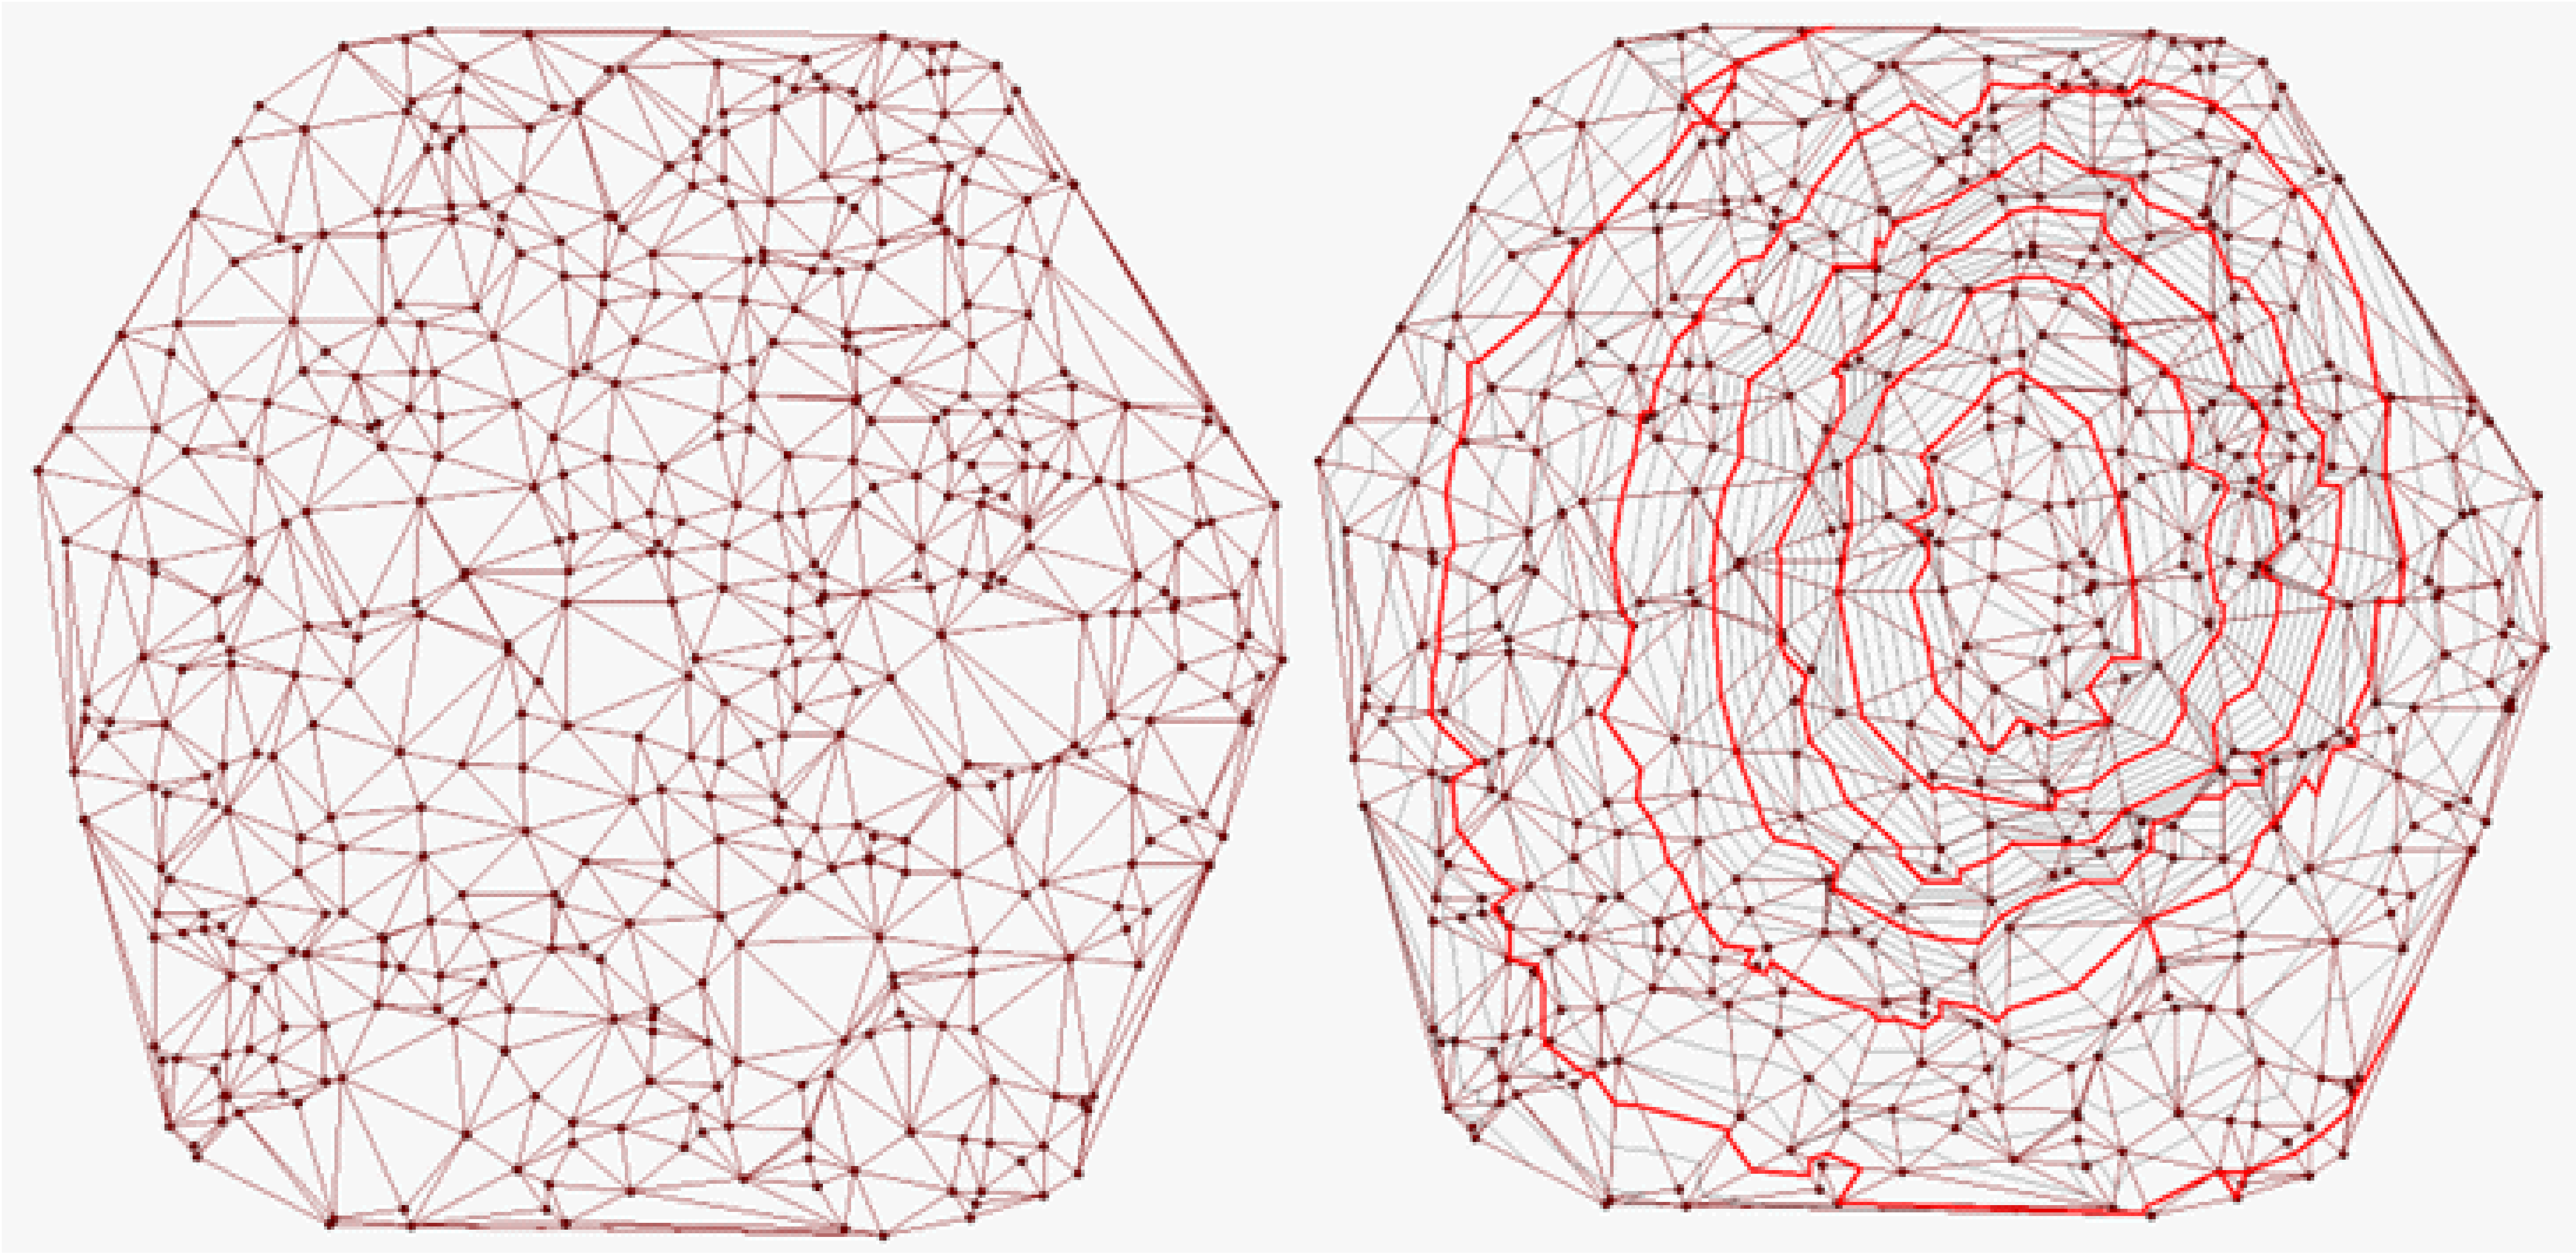
\includegraphics[height=80mm]{images/kupa_tri_vrst.PNG}\]
\[\textit{\footnotesize{Obr. 6 - Triangulace a tvorba vrstevnic pro kupu}}\]
\[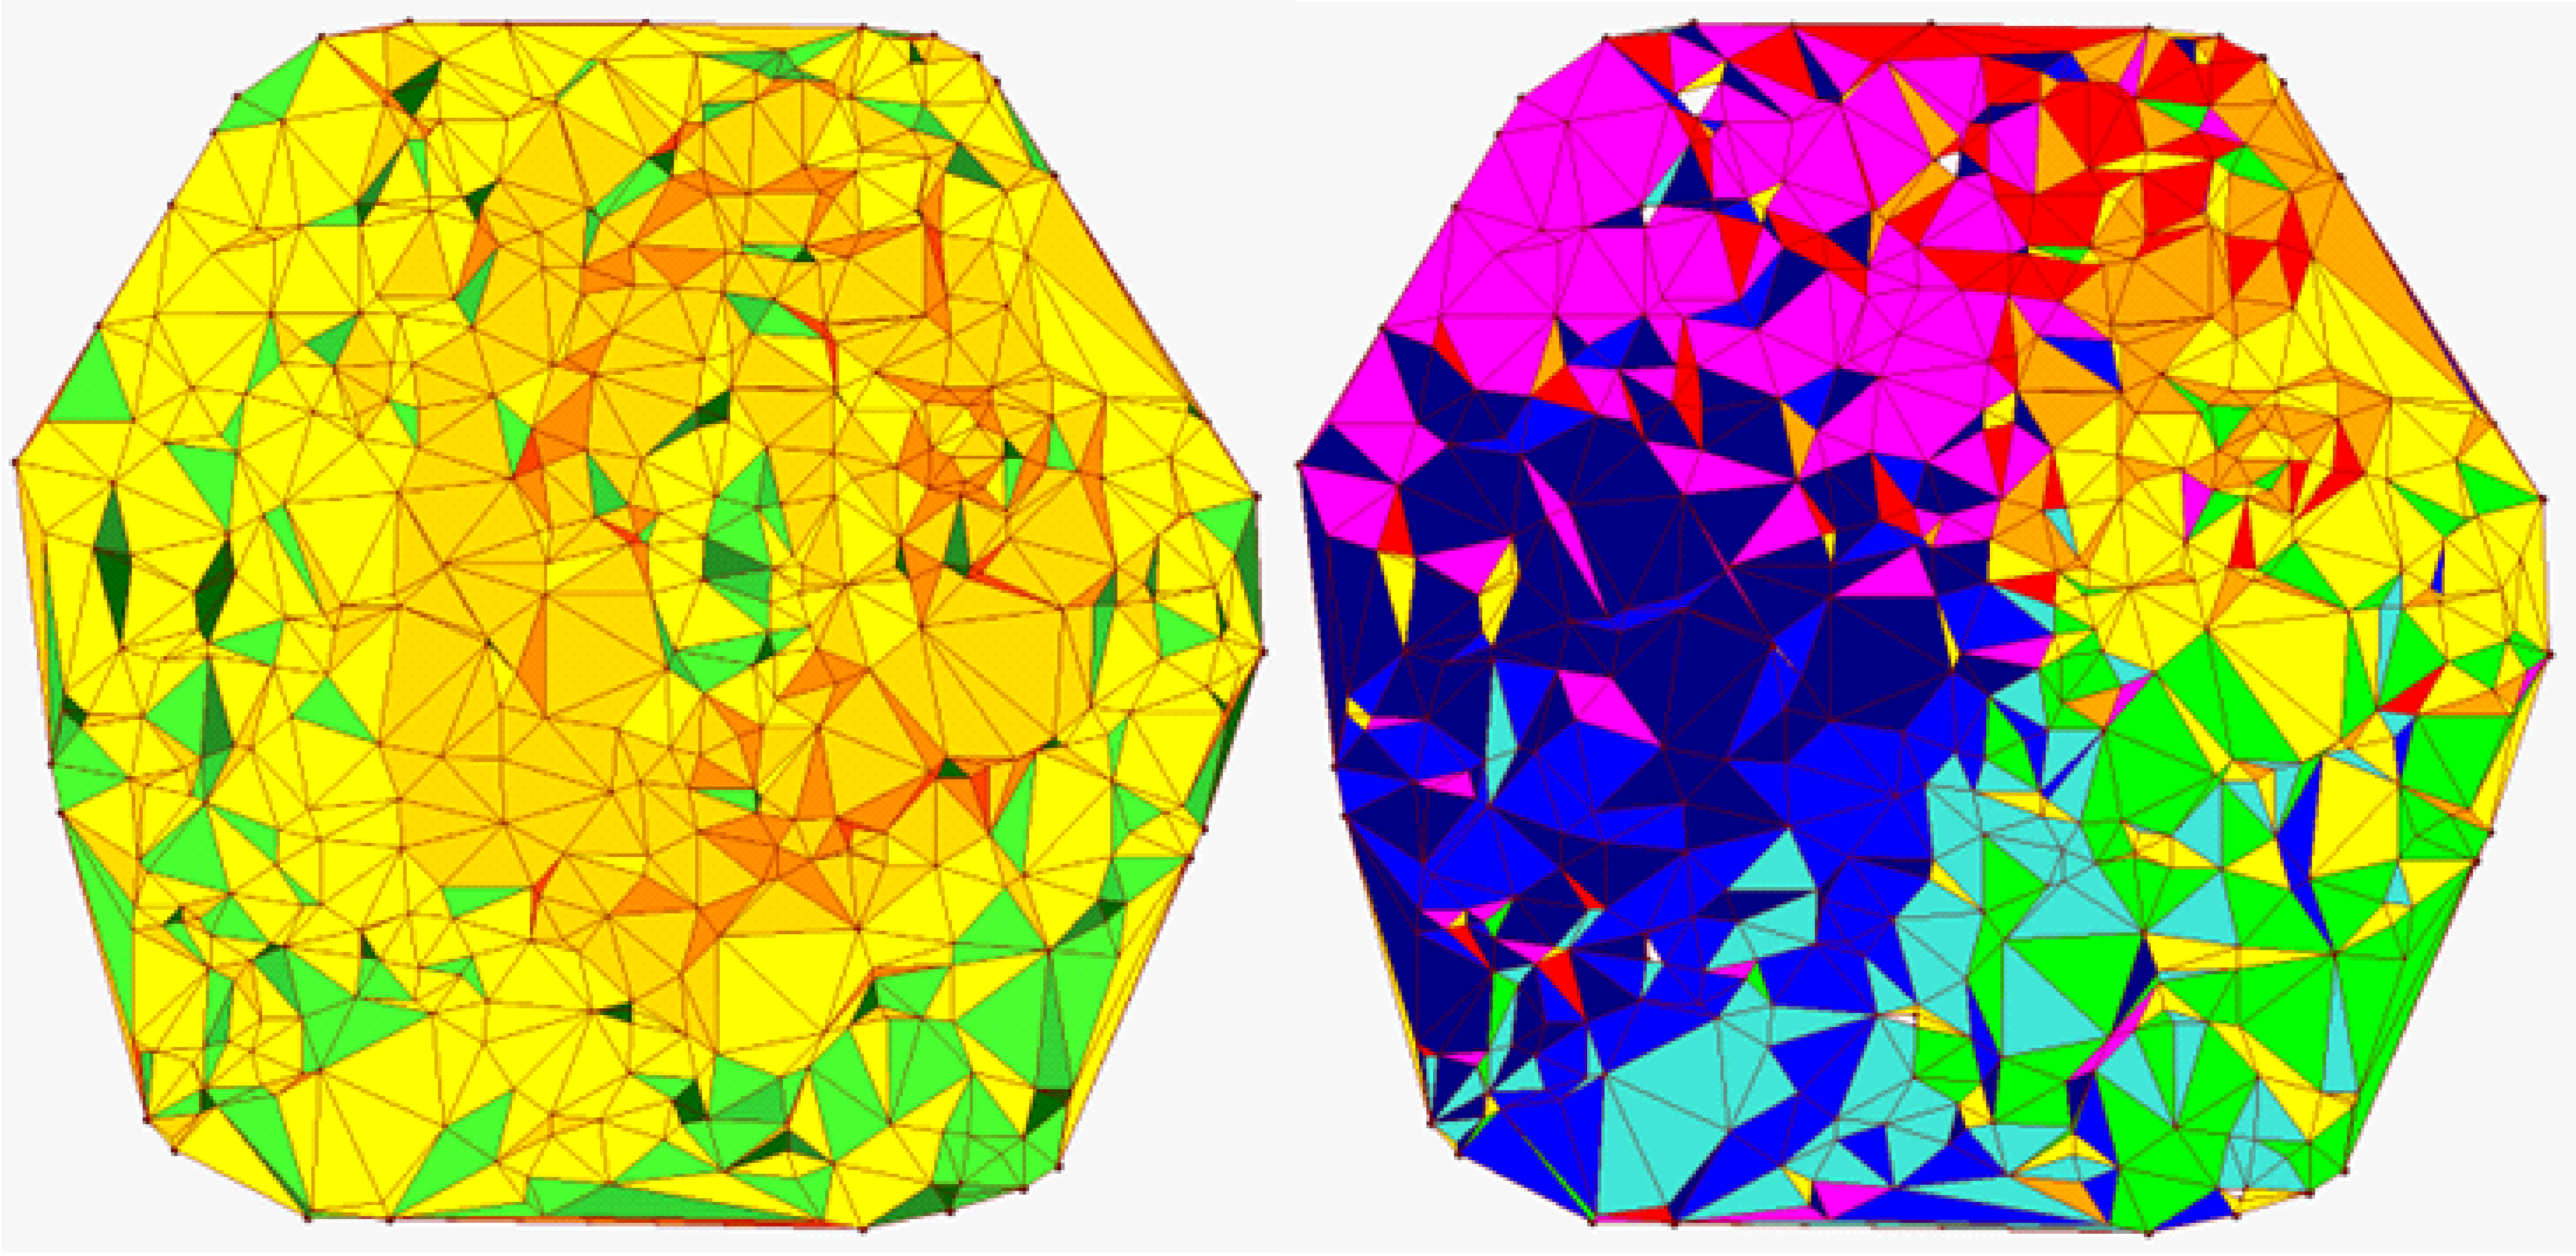
\includegraphics[height=80mm]{images/kupa_slope_aspect.PNG}\]
\[\textit{\footnotesize{Obr. 7 - Sklon svahů a orientace svahů pro kupu}}\]
U kupy při výpočtu všech 4 základní funkcí nedochází k žádným viditelným problémům.\\
\[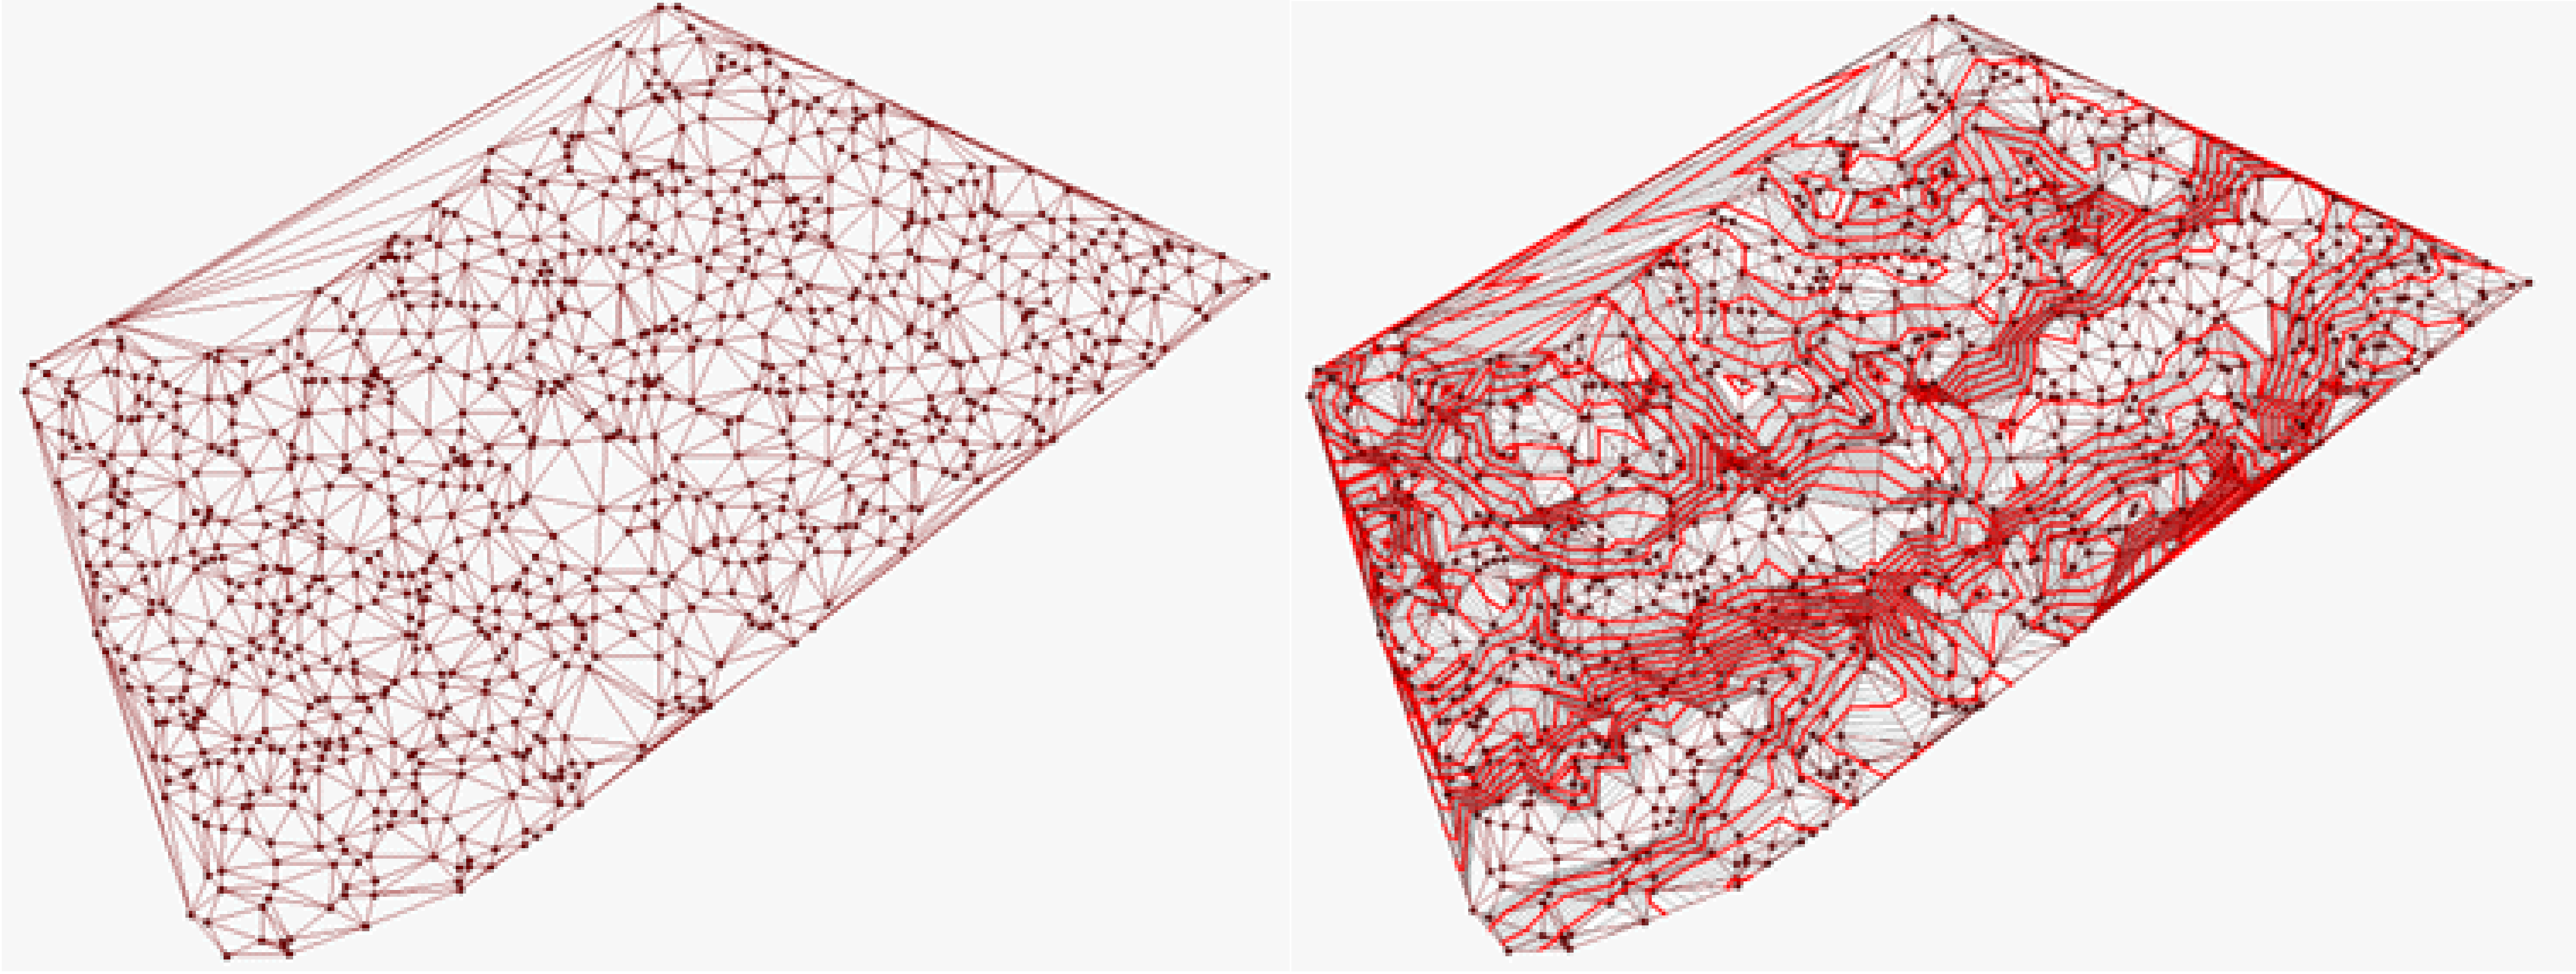
\includegraphics[height=61mm]{images/udoli_tri_vrst.PNG}\]
\[\textit{\footnotesize{Obr. 8 - Triangulace a tvorba vrstevnic pro údolí}}\]
\[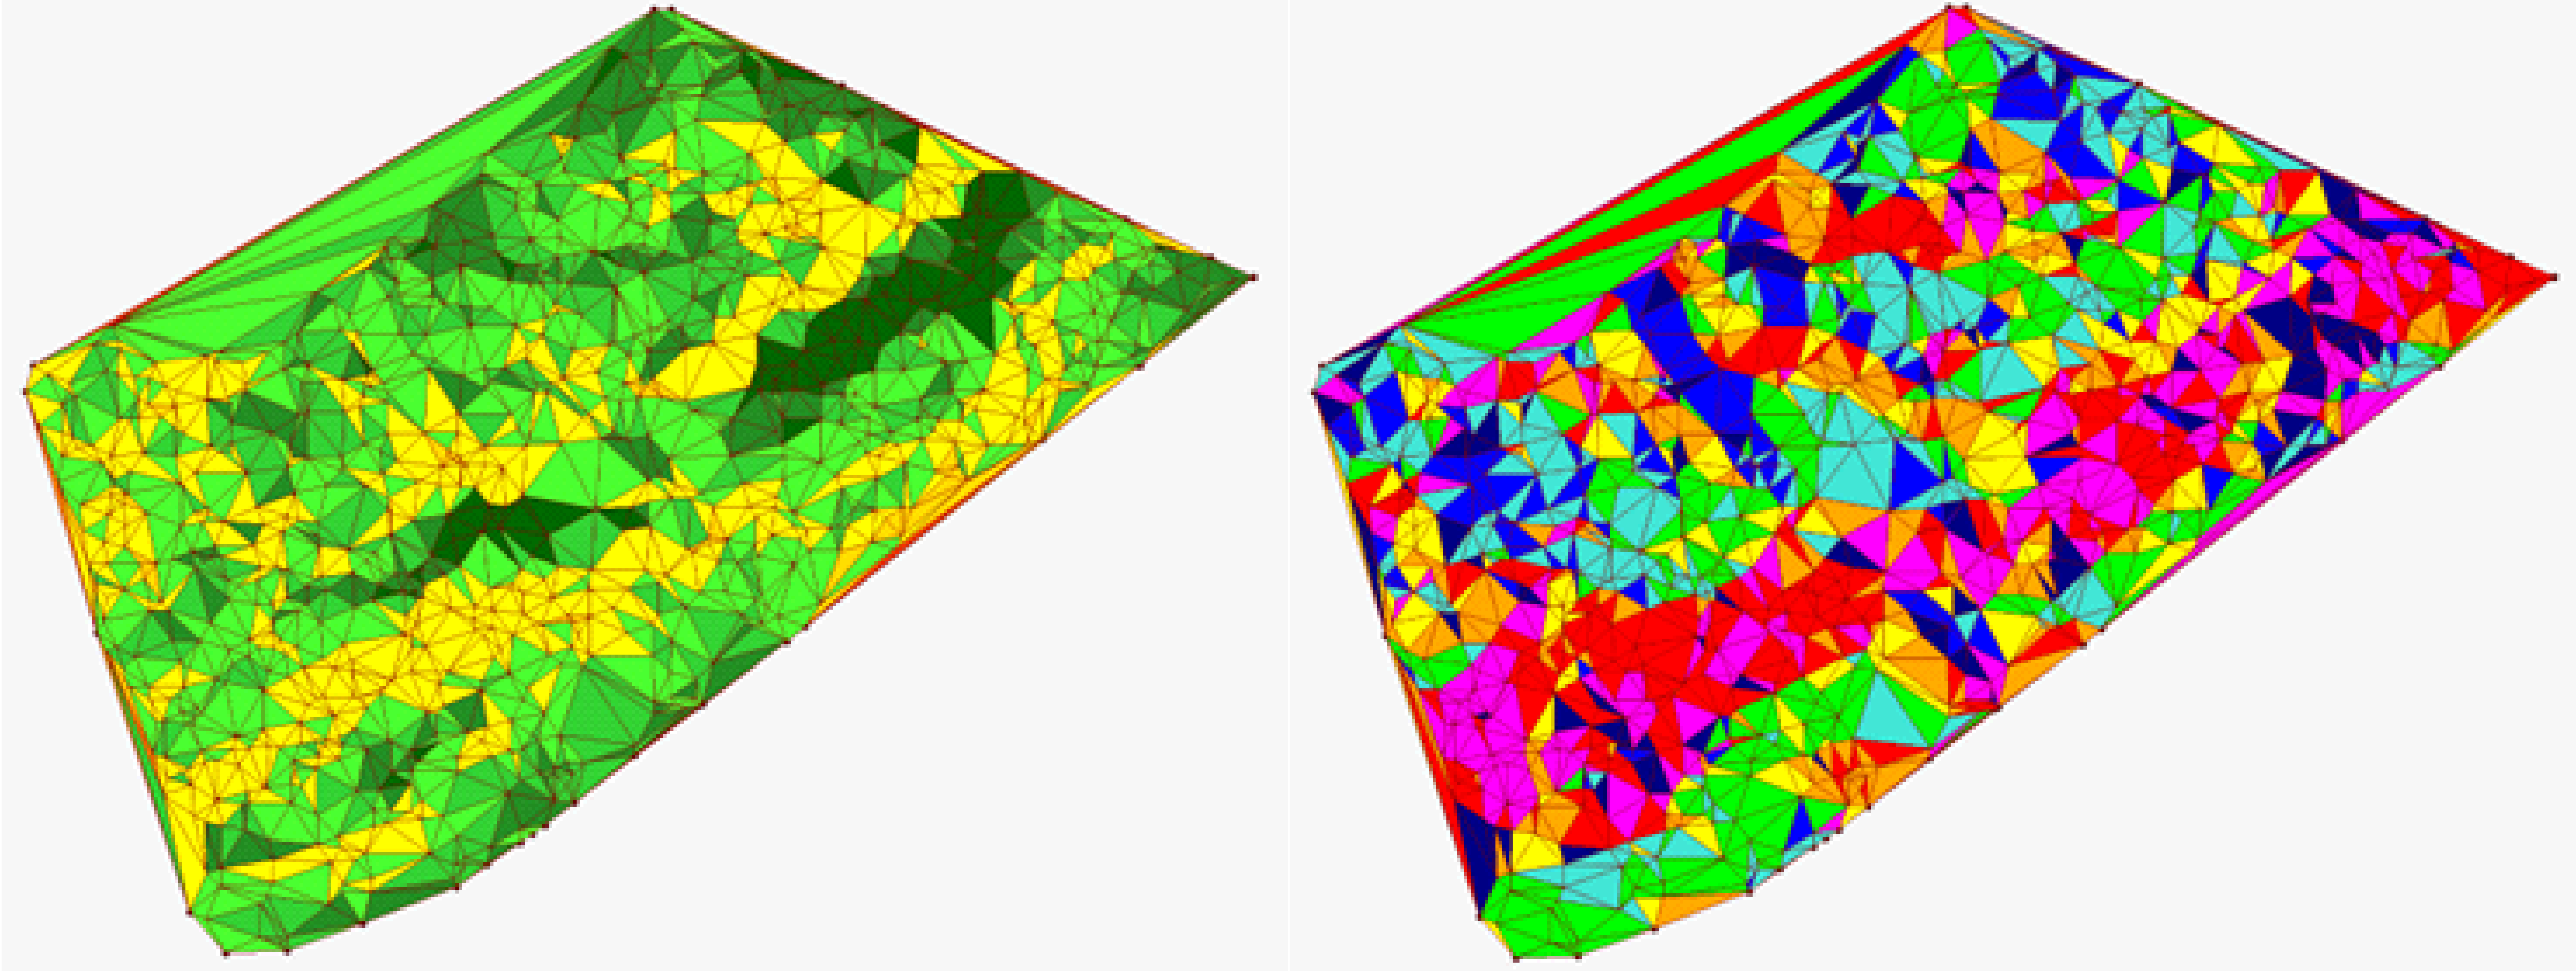
\includegraphics[height=61mm]{images/udoli_slope_aspect.PNG}\]
\[\textit{\footnotesize{Obr. 9 - Sklon svahů a orientace svahů pro údolí}}\]
Při výpočtu základních funkcí pro data reprezentující údolí první 3 funkce fungují bez větších potíží. Potíž nastává při výpočtu orientace svahu pro dno údolí. Zde je totiž svah blízký 0 a orientace je zde těžce vypočitatelná a skokově se mění u každého trojúhelníku.\\
\[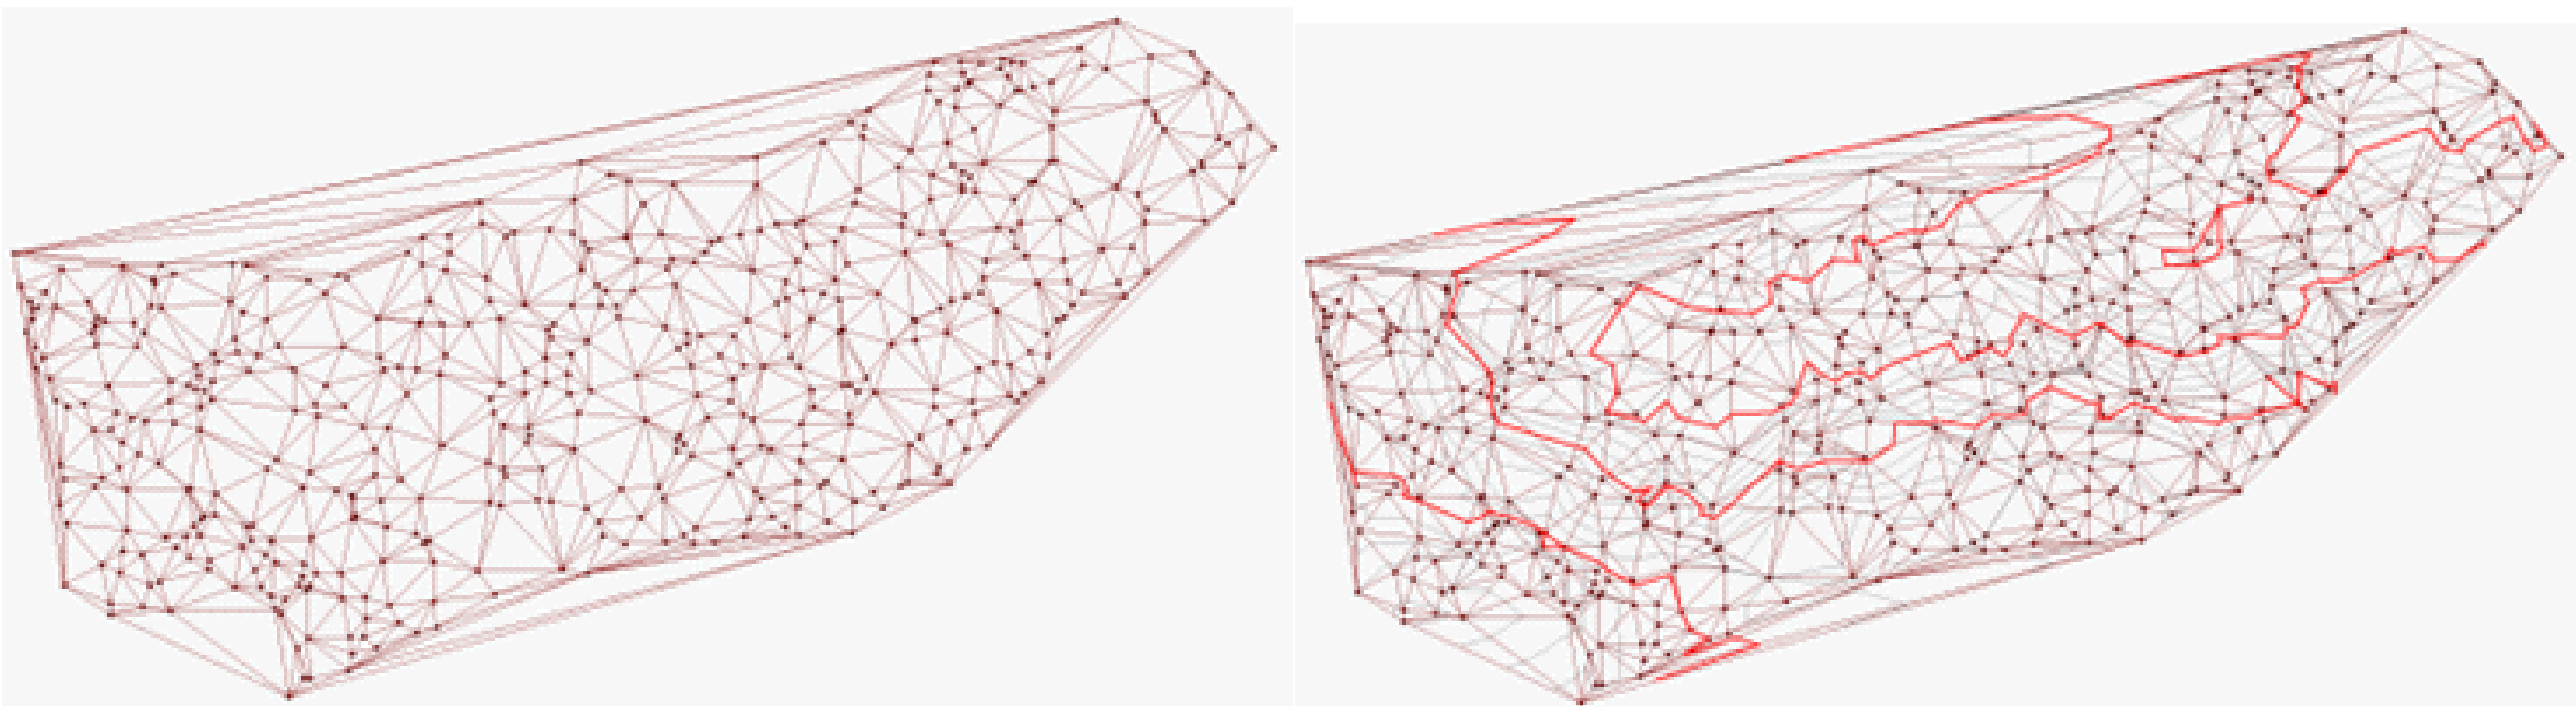
\includegraphics[height=44mm]{images/hrbet_tri_vrst.PNG}\]
\[\textit{\footnotesize{Obr. 10 - Triangulace a tvorba vrstevnic pro hřbet}}\]
\[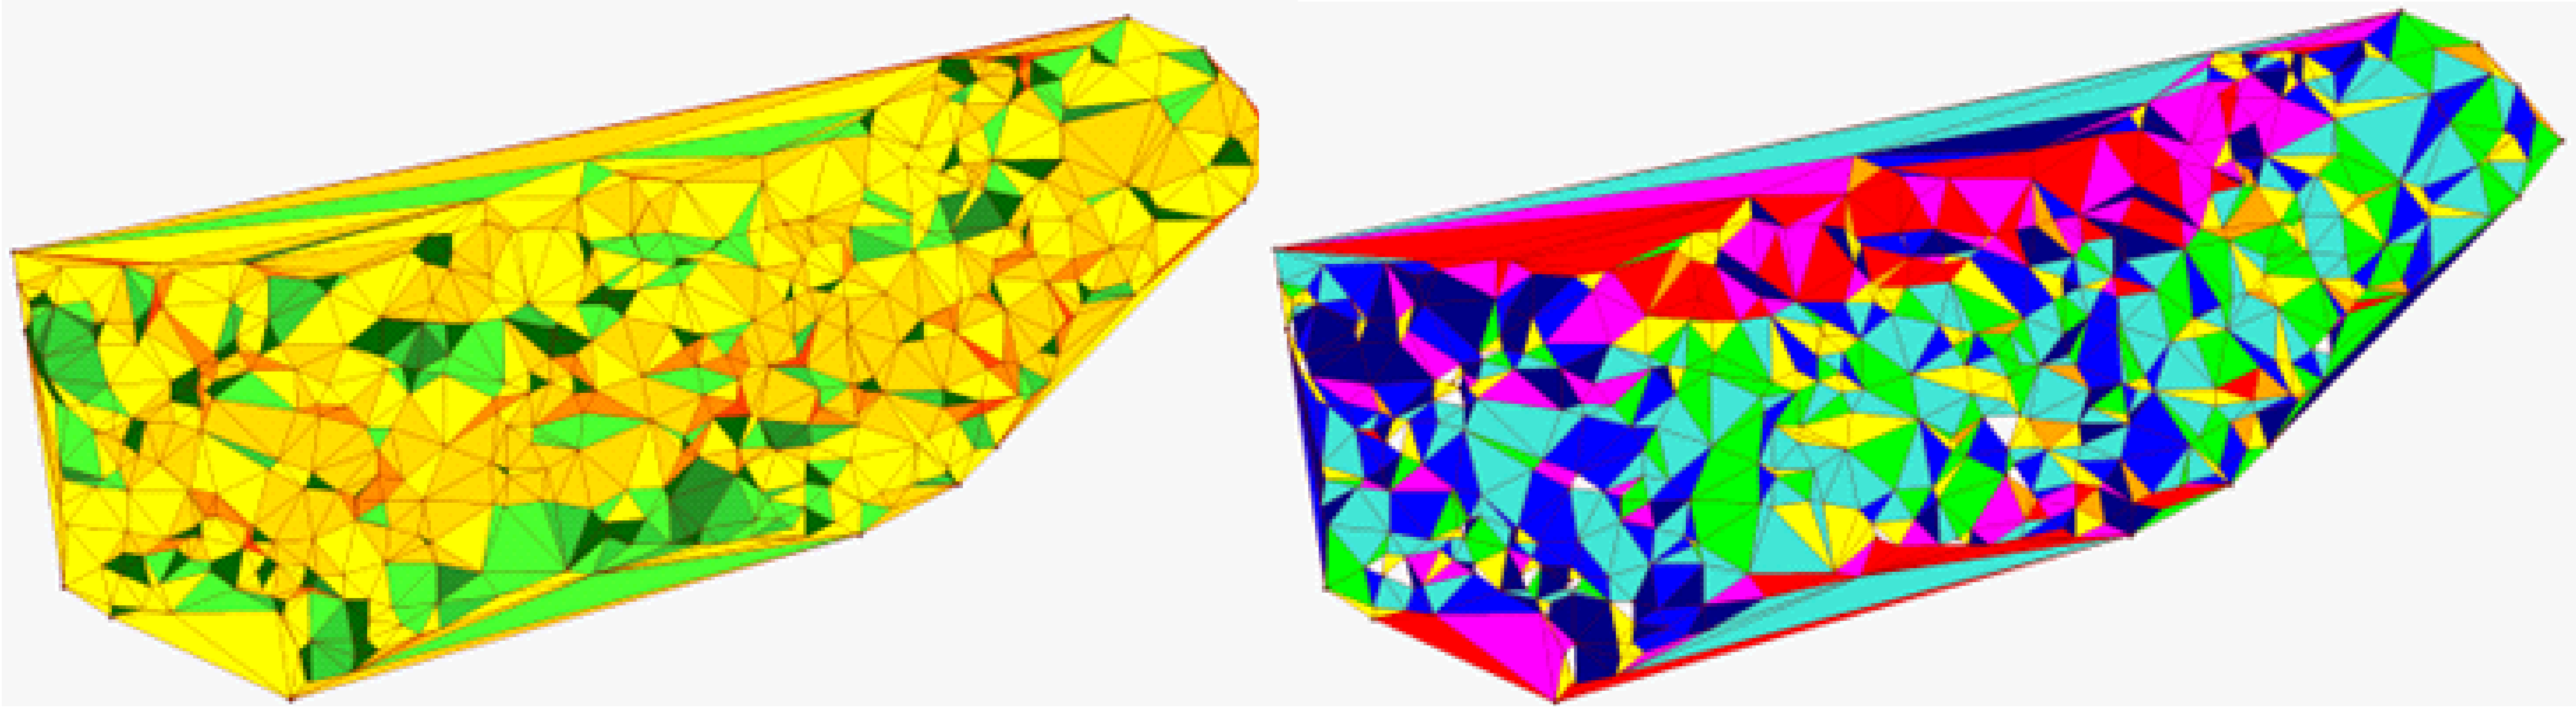
\includegraphics[height=44mm]{images/hrbet_slope_aspect.PNG}\]
\[\textit{\footnotesize{Obr. 11 - Sklon svahů a orientace svahů pro hřbet}}\]
U triangulace hřbetu a následného výpočtu sklonu, orientace a tvorbě vrstevnic je patrné, že ze zvolených 3 přírodních útvarů dopadly výsledky nejhůře. To však může být způsobeno nekvalitními daty. Data hřbetu by měla mít podobný problém jako data z údolí.\\
Nakonec byla funkčnost metod aplikována na umělá data (Obr. 12). Zde aplikovaná triangulace pracuje jen se 2D daty. U nich při pozvolných změnách nadmořské výšky není patrný nedostatek toho, že není brán v úvahu i třetí rozměr. Při prudkých změnách (např. terénní hrany) nastává problém a přesný průběh hrany zaniká, protože při tvorbě triangulace bylo na body nahlíženo jen v rovině x a y. Tyto problémy řeší datově závislá triangulace tzv. DDT.\\
\[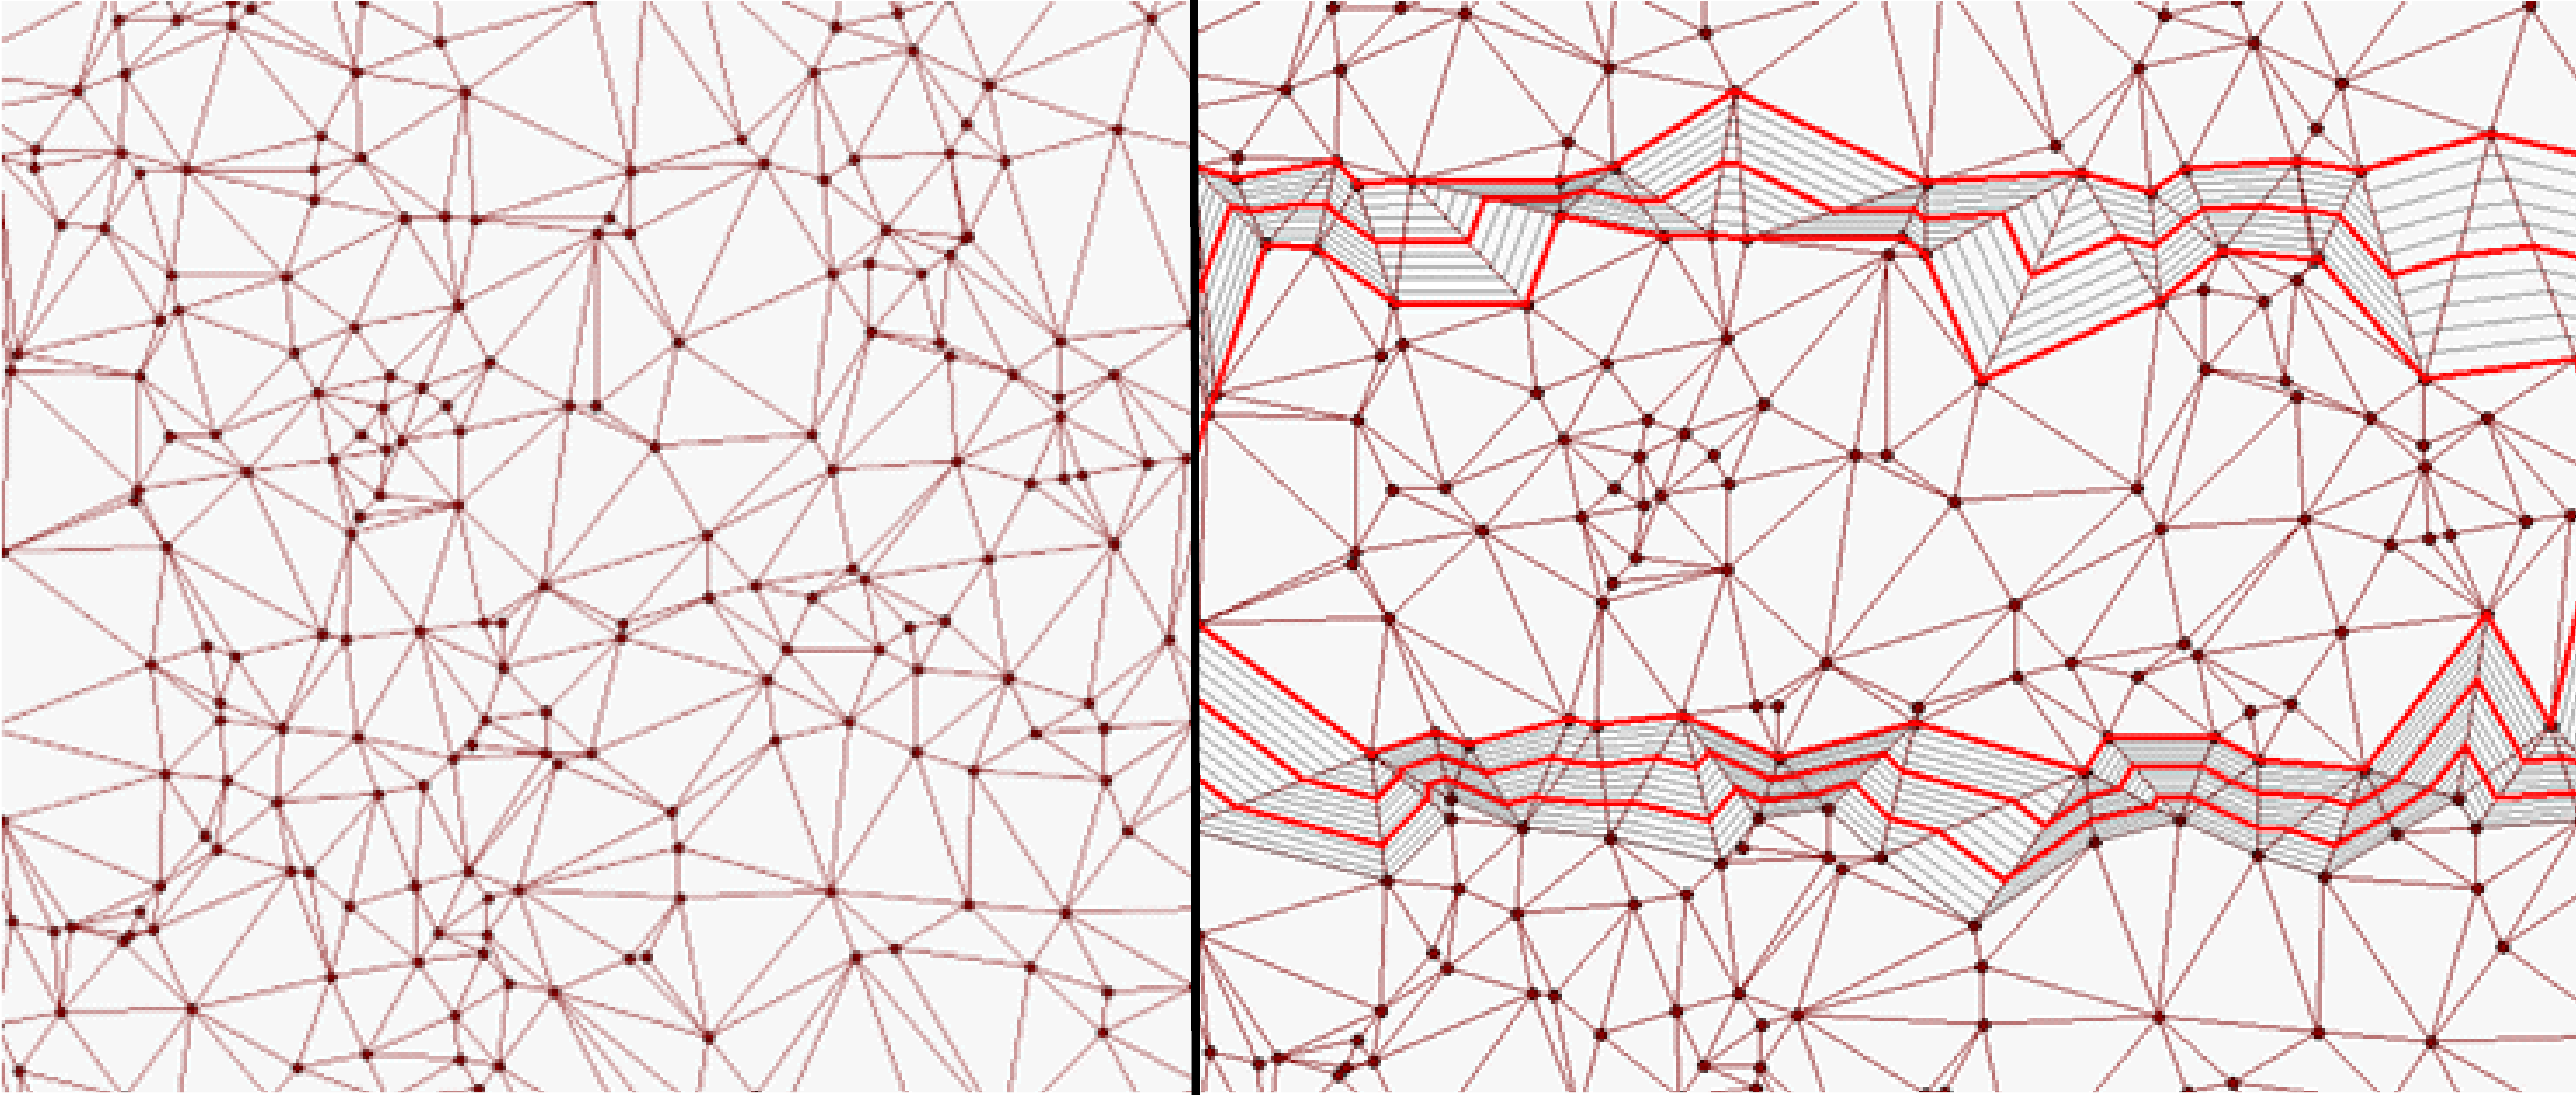
\includegraphics[height=68mm]{images/terenni_hrana.PNG}\]
\[\textit{\footnotesize{Obr. 12 - Syntetická data terénní hrany}}\]
Některé zde prezentované výsledky a chyby mohou být zkresleny tím, že metody nebyly testovány na vhodných a podrobných datech. Tento problém je nejvíce patrný u testování na datech reprezentující hřbet.
\clearpage
\newpage
\section{\large{Závěr}}
Program zpracovává bodové mračno, které mu je předáno ve formátu \emph{.shp}, který nese souřadnici z ve 4. sloupci atributové tabulky. Program by mohl být rozšířen o volbu sloupce, kde se nachází informace o nadmořské výšce bodů.
\clearpage
\newpage
\section{\large{Zdroje}}
BÆRENTZEN, J. A., GRAVESEN, J., ANTON, F., AENÆS, H. (2012): Triangle Mesh Generation: Delaunay Triangulation. In: J. A. Bærentzen, J. Gravesen, F. Anton, H. Aenæs (ed.): Guide to Computational Geometry Processing - Foundations, Algorithms, and Methods. Springer, Londýn, 330 s.\\
\\
DELAUNAY, B. (1934) Sur la Sphère Vide. A la Mémoire de Georges Voronoi. l'Académie des Sciences de l'URSS, Otdelenie Matematicheskih i Estestvennyh Nauk, vol 7., s. 793-800.\\
\\
DE BERG, M., CHEONG, O., VAN KREVELD, M., OVERMARS, M. (2008): Computational Geometry: Algorithms and Applications. Third Edition. Springer, Berlín, Heidelberg, 388 s.\\
\\
WEISSTEIN, E. W. (2016): Slope. MathWorld - A Wolfram Web Resource.\\
\end{document}
